\section{Ergebnisse und Diskussion}

\subsection{Durchlassfilter}
Beim Aufzeichnen der Spannungskurven für verschiedene ohmsche Widerstände fiel auf, dass die Maxima im Vergleich zu denen der Theoriekurven berechnet nach \eqref{form:durchlass} deutlich zu klein waren. (siehe Abb. \ref{plotdurchlass+R_ges}) Dabei wurde auch der an weiteren Bauteilen, hierbei vor allem die Spule, abfallende Widerstand berücksichtigt. Dieser wurde zuvor zu 3,0 $  \Omega $ ausgemessen.
\begin{figure}[h]
        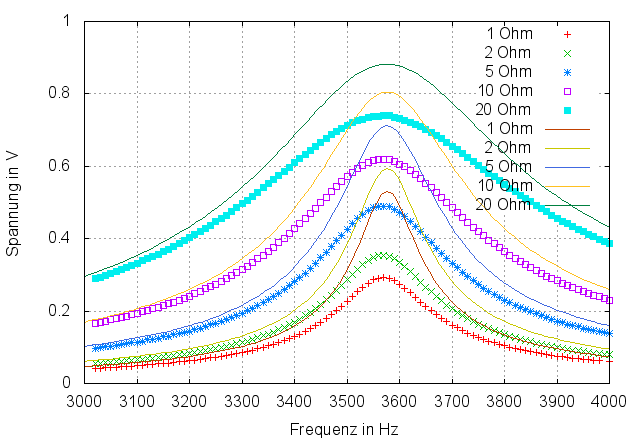
\includegraphics[width=.9\textwidth]{images/plot/durchlassfilter+theorie+R_ges.png}
\caption{Plot der Messdaten des Durchlassfilters unter Berücksichtigung des gemessenen Gesamtwiderstandes}
\label{plot:durchlass+R_ges}
\end{figure}
Abbildung \ref{plot:durchlass+R_ges-fit} zeigt die gleiche Messreihe, wobei hier über dem Gesamtwiderstand des Kreises als Variable gefittet wurde, um zu zeigen, dass der Gesamtwiderstand des Kreises um etwa 4 $\Omega$ größer ausfällt als wir durch Messungen am ausgeschalteten Schaltkreis messen konnten. Grund hierfür ist wohl schlichtweg zusätzlicher Widerstand, der sich als Übergangswiderstand bei den Steckverbindungen ausbildet, oder ein thermischer Widerstand in der Widerstandsbox.\\
Die geringen Abweichungen der Resonanzfrequenz von 50 Hz $\pm$ 1 Hz, die überdies hinaus zu sehen sind, könnten unter anderem auf ungenaue Kapazitäts- und Induktivitätsangaben zurückgeführt werden, fallen allerdings kaum ins Gewicht.

\begin{table}
\centering
\begin{tabular}{cc}
$R_{mess}$ in $\Omega$ & $R_{zus}$ aus Fit \\
\toprule 
1 & 11,48 \\ 
2 & 11.20 \\ 
5 & 10.70 \\ 
10 & 10.57 \\  
20 & 10.88 \\
\end{tabular}
\caption{Zusätzliche Widerstände aus Fit (siehe Abb. \ref{plot:durchlass+R_ges-fit})} 
\end{table}

\subsection{Sperrfilter}
Ähnlich verhält es sich mit den aus dem Betrieb der zweiten Schaltung als Sperrfilter entstandenen Kurven (Abb. \ref{plot:sperr}). Nach Berücksichtigung des ohmschen Widerstandes der Spule ergeben sich immer noch kleine Abweichungen zwischen Theorie nach Formel \eqref{form:sperr} und den Messwerten, die Resonanzfrequenz konnte nicht getroffen werden, sie weicht 15 $\pm$ 0.7 Hz von den Erwartungswerten ab. Hier scheint es ebenfalls am wahrscheinlichsten, dass die Induktivität der zweiten Spule mit 36 mH nicht korrekt ist, oder dass in anderen Bauteilen ungewollte Induktivitäten oder Kapazitäten auftreten.
\\
Der systematische Fehler wurde in beiden Versuchen nicht mit dargestellt, da er im Verhältniss zu den gemessenen Werten sehr gering ausfällt und die Graphen unnötig unübersichtlicher gestalten würde.
Der statistische Fehler konnte von Cassy nicht ausgegeben werden. Cassy mittelte die Messwerte automatisch über einen Zeitraum von 2 Sekunden.


\begin{figure}
	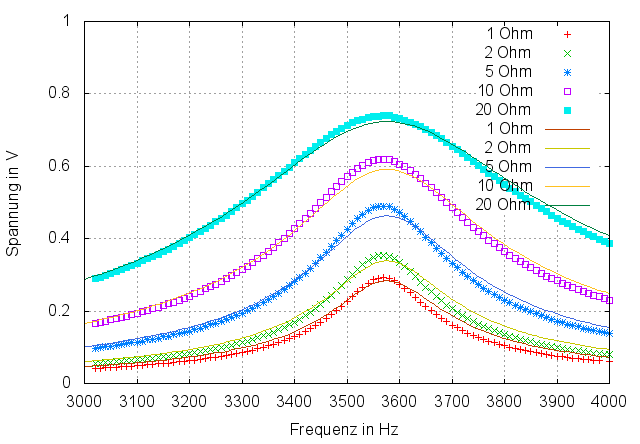
\includegraphics[width=.9\textwidth]{images/plot/durchlassfilter+theorie+R_ges-fit.png}
\caption{Plot der Messdaten des Durchlassfilters (Theoriekurven mit gefittetem Gesamtwiderstand)}
\label{plot:durchlass+R_ges-fit}

        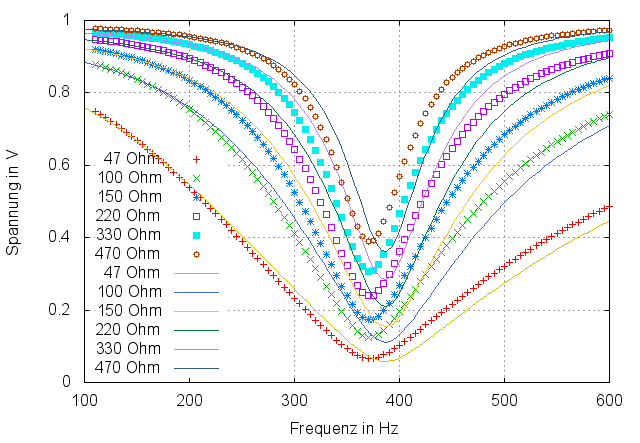
\includegraphics[width=.9\textwidth]{images/plot/Sperrfilter-mit-Theoriekurven-mit-R_L.png}
\caption{Plot der Messdaten des Sperrfilters mit (Theoriekurven mit gemessenem Widerstand)}
\label{plot:sperr}
\end{figure}

\subsection{Fazit}
Vergleicht man also die Theorie der behandelten Frequenzfilter mit den tatsächlich gemessenen Ergebnissen, so stimmen beide vor allem in qualitativer Hinsicht gut überein. Durch Ersetzen von etwa der Widerstandsbox durch einen Schichtwiderstand, eine Reduktion des Widerstands der Spule sowie durch Löten der Kontake an Stelle von gewöhnlichen Steckverbindungen müssten darüberhinaus deutliche Verbesserungen möglich sein, was die Höhe des Spannungsverlaufs und dessen Abweichung von der Theorie betrifft. 
Darüber hinaus müsste es durch die Verwendung genauer ausgemessener Induktivitäten und Kapazitäten auch möglich sein, einem idealen Frequenzfilter näher zu kommen. 
